\begin{figure}[b!]
\centering
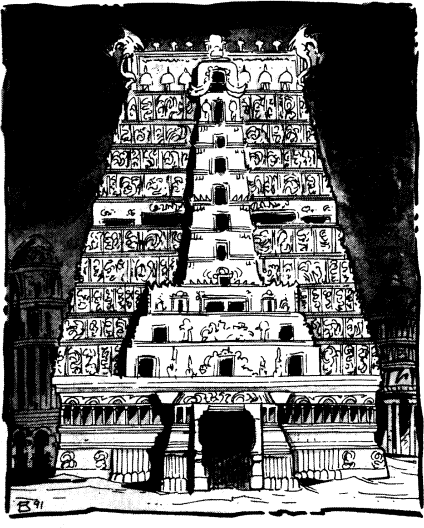
\includegraphics[width=\columnwidth]{images/tyr-1.png}
\par\textit{\small\textcopyright Wizards of the Coast, 2020.}
\end{figure}

\City{Tyr}
{15,000 (70\% humans, 10\% dwarves, 9\% half-giants, 6\% muls, 3\% elves, 1\% half-elves, 1\% other).}
{Iron, silk.}
{Common, Dwarven, Elven, Tyrian.}
{
	Located in a fertile valley in the foothills of the Ringing Mountains, it was the first city-state to successfully revolt against its sorcerer-king. King Kalak ruled Tyr until he fell to a group of heroes led by the gladiator Rikus, the wizard Sadira, and Agis of the noble house of Asticles. With Kalak dead, the High Templar Tithian stepped forward to take his place as king. Tithian received the backing of Rikus and the others, for the templar promised to free all Tyr slaves and institute other sweeping reforms---promises he actually kept. Tithian had his own agenda, of course, which slowly played out over the decade he held the throne.

	The new king created the Council of Advisers and gave members of the most important groups in Tyr a role in the city's government. Councilors were drawn from all ranks of society and worked diligently to pass laws that would strengthen Tyr's newfound freedom. Tithian allowed the Council to operate independently and virtually run the city while he sought the means to become a true sorcerer-king.

	Urik tried to capture Tyr's iron mines less than six months after Kalak's death. The resulting battles made Tyr's leaders realize how necessary a strong military was, and how important it was to resume iron production and get trade and commerce back on an even keel. During his reign, the new king also faced the problem of finding a way to overcome the Dragon's levy, had numerous skirmishes with raiding tribes, and battled angry giants intent on plundering the city. The Council struggled to stay together in the face of secret agendas and conflicting partisan interests. The templar revolt of Free Year 3 shut down the bureaucracy and public works for nearly two months until those who swore new oaths to abandon the old ways and support the tenets of Free Tyr were given more representation in the Council. The artisan strike of Free Year 6 lasted almost four months, and then ended in increased wages for basic services. Agis and the Council handled most of these crises in one way or another, for Tithian was much too busy to get involved in what he considered to be the chores of government.

	Today, in its twelfth year of freedom, Tyr faces new challenges. Agis of Asticles is dead, so his wisdom and honor can no longer guide the Council of Advisers. King Tithian's rule has come to an end. His ambitions led to his downfall, for he is trapped in the Cerulean Storm (though only a few people know of his true fate). The general populace believes that Tithian died fighting to keep Tyr free, thanks to the tales told by Rikus and Sadira. The heroes decided to keep Tithian's current state a secret, fearing that ambitious defilers might try to free him in order to gain power and prestige. Can Tyr's freedom take root in the Tablelands in the wake of these events, or will it be blown away in a devastating Tyr-storm?

	Tyr citizens remain as untroubled by modesty as they were in the days of Kalak. The less a person has to wear in the heat of the day, the better. Most wear loose-fitting cotton tunics gathered at the waist with wide, colorful belts. Others wear loincloths and vests. Light gauze or silks are draped over heads and exposed flesh to protect the skin from the blistering sun. Turbans and other forms of light headgear often finish off a Tyrian's attire.
}
{
	Four months into its twelfth year as a free city, Tyr must deal with the environmental and social conditions left over from the past decade. The Great Earthquake, for example, struck while most of Tyr's beloved heroes and its king were away. It fell to the remaining members of the Council of Advisers to pick up the pieces. Though the rumbling ground made for a terrifying period of time, Tyr escaped the disaster relatively unscathed. There was some structural damage and a small number of deaths, but most of these occurred in the Warrens. The comparatively weak and dilapidated buildings in this part of the city buckled when the quake hit, burying the residents beneath rubble and debris. Ironically, if the quake had struck during Kalak's reign, even less deaths would have occurred. In Kalak's day, the Warrens were mostly unoccupied. It's only since the First Edict freed the slaves that the Warrens have been filled to overflowing with the new crop of free citizens.

	The earthquake caused other damage. Cracks appeared in the city wall, and a whole section of the wall near the Grand Gate collapsed. Minor damage can be seen throughout the rest of the city, but the most noticeable appears on Kalak's Ziggurat. Great cracks riddle one face of the tower, while another face has collapsed into a heap of rubble. The client villages that dot the valley endured the worst of the quake's effects, however. One village was leveled by the quake, and others were pounded by rockslides that cascaded out of the mountains.

	Beyond the death and destruction, the worst aspect for the city is the refugees. Intelligent races and a wide variety of creatures and monsters have fled the mountains, flooding the valley in search of a safe haven. This, in turn, has sent villagers to the city gates, seeking protection from the ravaging hordes.

	What with the Great Earthquake, the periodic aftershocks that visit the city, and the violent Tyr-storms that occasionally sweep the land, the populace has turned into a frightened mob. Not everyone has succumbed to these base fears, of course, but a significant portion has lost control-the Council desperately needs to find a way to calm the people and restore order. A particularly vocal group claims that Kalak has returned to gain vengeance against the city, calling for open worship of the sorcerer-king to appease his wrath. Others have been trying to placate the elemental spirits of earth, hoping that they'll spare Tyr from their ground-shaking anger. Then there are those who seek to take advantage of the misfortune, looting shops, robbing nobles, and generally taking what they want and need by force of arms. These violent mobs are concentrated in the Warrens, but they sometimes range into other parts of the city to sow mayhem and destruction.

	The Council of Advisers has been working overtime to address these problems, though first it had to deal with King Tithian's supposed death. It established the OverCouncil to rule in Tithian's place so that the business of government could continue.

	Second, it increased the size of the City Guard and commanded it to restore order. Things haven't returned to normal yet, but the situation is much better than it was in the days immediately following the Great Earthquake. Various subcommittees have been set up to handle damage control, to see to the fair distribution of water and supplies, and to handle the refugee problem -both those rushing into the valley and those fleeing the villages for the safer environs of the city walls.

	The situations in the other city-states have added to the general nervousness and apprehension hanging over Tyr. While Urik has sealed itself off from the rest of the Tablelands (except for the heavily armed trade caravans that set out and return at random intervals), Gulg and Nibenay have made a few overtures to the Council of Advisers. Both city-states have offered to aid Tyr, claiming that without a sorcerer-king to defend it, the city is vulnerable to all sorts of terrible dangers. The Council, naturally, has thus far graciously refused these offers. Draj and Balic have recently resumed trade with Tyr, but both cities have changed significantly since the reported deaths of their sorcerer-kings. In fact, though Sadira and Rikus assured the Council that the kings had been disposed of by Rajaat, rumors of their return continue to drift in with caravans, adventurers, and refugees. The worst tales come out of Raam, where confusion, madness, and ambition have given rise to anarchy. Tales of nobles being murdered in their homes, of templars being slaughtered in the streets, and of vicious invaders from a hidden city-state controlled by a king named Dregoth have made the Tyr citizens ill at ease and not quite confident that their leaders can protect them.

	Sadira recently convinced a significant portion of the Veiled Alliance to come out of hiding and join Tyr society. These wizards formed a new group in Tyr, called the Preservers. The Preservers were given a place on the Council of Advisers to reflect their new role in Tyr. Sadira, as their leader and as an important member of the Council, was assigned to the OverCouncil. These good wizards are developing plans and guidelines for helping the city in a variety of ways that adhere to their overall morals and code of ethics.
}
{
\begin{figure*}[b!]
\centering
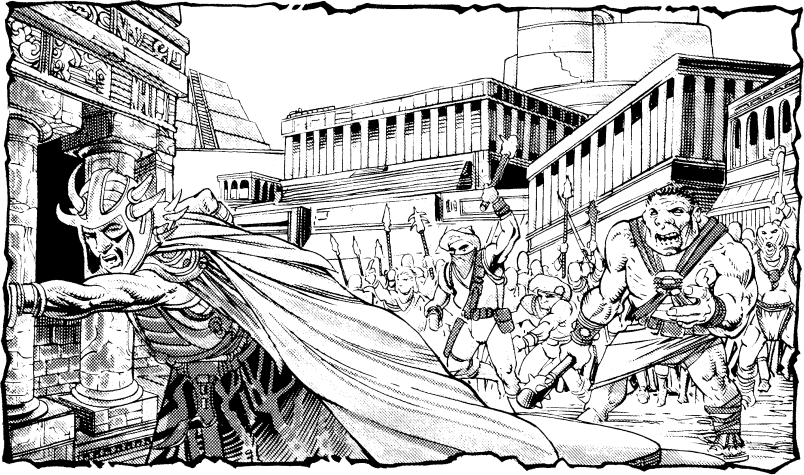
\includegraphics[width=\textwidth]{images/tyr-2.png}
\par\textit{\small\textcopyright Wizards of the Coast, 2020.}
\end{figure*}

	A Council of Advisers makes the laws of Tyr. The Council is divided into five distinct groups who together represent Tyr's varied citizenry. These groups are the Guildsmen, made up mostly of human and dwarf artisans and other professionals from Tyr's three trade districts; the Nobles, representing Tyr's aristocratic families; the Templars, who continue to handle administrative functions in the city; the Free Citizens, chosen from among the masses who were either slaves or paupers before Tyr's liberation; and the Preservers, the newest group admitted to the Council, consisting of members of the once secret and outlawed Veiled Alliance.

	When Rikus, Neeva, and Sadira returned with the news of Agis' and Tithian's death, it was resolved that the Free City shouldn't be burdened with another king. With no king to lead the city, the Council now oversees all aspects of government; a subcommittee made up of one member from each of the Council's divisions serves as an OverCouncil. This OverCouncil governs on a daily basis, while the entire Council of Advisers only meets three out of every fifteen days. The OverCouncil consists of the dwarf stonecutter Gar Bonehammer (NG male dwarf, expert 3) who represents the Guildsmen; Lady Laaj of Mycilen (LE female human, seer 6) for the Nobles; the High Templar Timor (LE male human, defiler 8) for the Templars; Rikus (NG male mul, gladiator 8/arena champion 10) who represents the Free Citizens; and Sadira (N female sun-touched half-elf, preserver 5/veiled one 5) for the Preservers.

	Surprisingly, the Council runs relatively smoothly. Some councilors posture for power and influence and partisan voting sometimes causes meetings to stall, but in general the Council has learned how to get the job done. Each division of the Council meets separately with its constituents to draft its own agenda before coming to a full session. Then the councilors do their best to get their own projects pushed through the voting process while trying to keep in mind the welfare of Tyr as a whole.

	While the Council deals with the big picture, the templars continue to fill the administrative roles they have long been associated with. Since the loss of their spellcasting abilities, it has become doubly important for this division to demonstrate why Tyr needs them. The tangled bureaucracy has been reformed, but it still exists.

	Without the templars to turn the massive wheels of government, Tyr's infrastructure would have collapsed long ago. High Templar Timor (who hides his status as a defiler) serves as the Minister of Tyr, overseeing the various Senior Templars who run departments like Fields, Finance, Public Works, Water, and Trade.
}
{
	\textbf{Free Wizards}: With preserver magic no longer outlawed in Tyr, Sadira convinced a number of preservers to come out of hiding and openly proclaim themselves to the city. As a group the free wizards are not a strong cohesive group. Individual free wizards pursue their own goals, whether in the political arena or merchant activities. Only the desire to instruct the populace in the differences between preserving and defiling magic and to build the public's trust in them unites the group.

	\textbf{House Vordon}: Under the last years of Kalak's reign, House Vordon had fallen from its position as one of the most powerful merchant houses in the Tablelands. Since the fall of Kalak, House Vordon has returned to a position of respect among its peers. The House's return to profitability is fueled by its specialization in the iron trade from the mines of Tyr.

	Thaxos Vordon is head of House Vordon. In the last ruinous days of Kalak's reign, Thaxos began a plan to overthrow the mad king. However, Kalak's demise at the hands of Rikus and the heroes of Tyr stopped him from going forward with the plan. In the years since, Thaxos has become convinced that he should become king of Tyr, and has refined the plan he originally developed for Kalak's overthrow. A number of dummy merchant houses have been created and large numbers of mercenaries hired as part of this plan. Unbeknownst to all but the highest members of House Vordon, Thaxos now has an army scattered at outposts throughout the region, waiting for his orders.

	\textbf{The Veiled Alliance}: The Veiled Alliance remains active in the wake of this new age of wizardly openness. Matthias Morthen (LG male human, preserver 8/veiled one 10) continues to lead a small number of preservers who feel that secrecy must be maintained until all of Kalak's defilers have been eradicated and the citizens of Tyr learn to deal with the responsibilities of freedom. Besides, Morthen doesn't like or trust Sadira, whom he believes has often approached the moral line between defiling and preserving magic (if not actually crossed over it) in the course of defending Tyr. He believes that the Veiled Alliance must continue, if only to serve as a balance for a wizard whose powers and motivations he doesn't fully understand.
}
{
	\textbf{Hidden Village (Thorp, 250)}: Established by the slave tribe known as the Free, the Hidden Village sits in a remote crater in the foothills of the Ringing Mountains between Tyr and Urik. Originally the tribe survived by raiding as most slave tribes do. Now the tribe has advanced into a small trading house. The villagers have developed such a strong relationship with Tyr that they have become a client village of the free city.

	\textbf{Kled (Village, 450)}: Kled is a Dwarven community that has ties to Tyr. Possibly the largest Dwarven community in the Tablelands, Kled was built near the ruins of the city of last Dwarven kings, Kemalok.

	\textbf{Mira's Halo (Thorp, 50)}: Mira's Halo is a merchant outpost owned by House Qual, one of House Vordon's dummy trading houses. The outpost is used in the iron trade between Tyr and Urik. The name of the outpost comes from an unusual rock formation nearby.
}
{
	\textbf{The Elven Market}: The Elven market is located inside the Warrens. Several nomadic Elven tribes trade at the market regularly, bringing a wide range of goods and curiosities from across the Tablelands. Many tribes own a building or two that borders on the square. Others take ownership of unoccupied buildings for the duration of their visit in Tyr. Anything can be found in the Elven market, legal or illegal. The customer just has to know the right people to ask. The market has a reputation for pick pockets and dubious merchandise, but people come from all over the city in order to find items not available anywhere else in Tyr.

	\textbf{Gladiator Stadium}: The Gladiator Arena of Tyr is the second largest building in the city, with only the ziggurat, which looms over one end of the stadium, being larger. The stadium's rectangular floor is some 90 meters long and 24 meters wide. The floor is of a hard packed sand with a reddish hue, which Tyrians say is caused by the spilling of the lifeblood of a thousand fallen gladiators. The stadium is unique in the Tyr Region as it has upper and lower seating sections. The upper section is generally referred to as ``The Sun Seats'' because of the lack of shade, and is open to the general populace. The crowd in the upper section is more raucous and enthusiastic than in the lower section. Seats in the lower section cost more and are traditionally used by merchants, and nobles.

	Despite the end of slavery in Tyr, gladiator matches are still held in the stadium. Now the bouts are not fought to the death and are open to any who wish to participate.

	The gladiator matches are only held on festival days. The remaining time, the arena floor is used for an open air market. A monthly array of tents and stalls cover the sandy floor in drunken rows. Traders who operate in these stalls offer a wide variety of legal and illegal goods and services.

	\textbf{Golden Tower}: The Golden Tower was the imperial home of the King of Tyr. Both King Kalak and King Tithian ruled from the Tower. Constructed of a rare golden granite, the tower gleams harshly during daylight. The only public entrance to the tower is to cross Tower Bridge from the Observation Tower. The public receiving areas are on the top floors, with the King's private chambers on the levels below. These included the King's library, an enormous collection of scrolls and books, many from ancient times.

	\textbf{Iron Mines}: Tyr's iron mines are the largest in the Tablelands and help the city exert leverage over the other cities in the region. The iron mines are located two days, travel northwest of the city. Death has always surrounded the mines, from cave-ins to the ``hej-kin's curse.'' The iron ore is transported to Tyr in heavily guarded caravans.

	\textbf{Kalak's Ziggurat}: The ziggurat built by Kalak still towers over the squalor of the city from its center. The ziggurat is a stepped pyramid with each level finished in a different colored glazed brick. An enormous staircase runs straight from the base to the summit of the ziggurat. Since Kalak's fall, the ziggurat has fallen into disrepair. The Great Earthquake has exacerbated this, causing an entire face of the pyramid to collapse. Great cracks riddle another face of the tower, causing concern that more of the pyramid may crumble soon. Few have dared enter the ziggurat since Kalak's death and it has become the focus of numerous rumors and frightening stories.

	\textbf{School of Thought}: The School of Thought is the only major organized institution for the study of psionics in Tyr. The school was founded a little over 30 years ago by the noblewoman Chessia. Chessia provided the funds to establish the school and made contributions to help the school operate over the years, but she is not involved running the school. The current headmistress of the School of Thought is Sycia Strimmen (NG female human, telepath 7/psiologist 9), a young and enthusiastic woman with considerable charm. She has been the headmistress for almost nine years now, since the previous headmaster, Thanik Arkos, disappeared from the school after murdering one of the master instructors. Sycia is very organized and well liked by students and instructors alike.

	\textbf{Shadow Square}: Shadow Square is a small entertainment district in the Warrens near Kalak's Ziggurat. Five lanes end at the small plaza around which sit six wineshops, a gambling house, and two hostelries. Most business in the square happens between sunset and dawn.

	\textbf{UnderTyr}: The site the city of Tyr was built on has been inhabited for thousands of years. The current city sits atop the ruins of these previous civilizations. An undercity of interconnecting byways, crumbled buildings, and dilapidated courtyards exists under the streets of modern Tyr. From buildings used as businesses to former residences and temples to forgotten gods all make up the structures of UnderTyr. It is not possible to travel from one side of the city to the other through UnderTyr. Instead pockets exist throughout the city. The location of the eight largest pockets is scattered and unconnected across the city. With names such as the Sorrows, Elven River, and Merchant's Maze, these underground locations provide opportunities for the brave or foolish. Many strange and wondrous items can be found in UnderTyr, as can dangerous creatures and malicious entities.

	\textbf{The Warrens}: The Warrens sprawl across the northern quarter of the city. The slum is filled with dilapidated structures and trash dumps. The district is filled to overflowing with the poor, mostly ex-slaves. Many are out of work, and the desperate and ambitious have chosen to prey on their neighbors. Gangs roam the Warrens targeting anyone who looks like they might have a ceramic piece. Templars and the city guard rarely patrol the Warrens anymore for fear of being overrun by the mob. Parts of the Warren are said to be cursed. Other buildings are said to be haunted or the lair of some wild beast. Anyone who enters the Warrens does so at their own peril.
}
{
	\item Slavery is outlawed in Tyr, but a group of slavers has set up a network to kidnap citizens of Tyr and sell them as slaves in other cities. The slaver network is elaborate, involving snatch teams that kidnap the victims, nobles whose estates are used to hold the captives, templars who look the other way, an Elven tribe that smuggles the slaves out of the city, and a merchant house, perhaps House Shom, that transports the captives to other cities where they are sold.
	\item Is the shadow of Kalak's ziggurat deadly? Rumors fly that ever since King Tithian's death, people are suddenly dropping dead while standing in the ziggurat's shadow. Those living close to the ziggurat are fearful of falling under what they have named Kalak's Curse. Many are fleeing, but no one knows what is causing the deaths.
	\item The elderly noblewoman Prisella Obstrunia is unlike many of her fellow nobles. Since the slaves were granted their freedom she has come to regret her past participation in the practice, and seeks to make amends somehow as she nears the end of her life. One of her former slaves, Raxenth, has remained with her as a servant and become a friend. When slavery was still in practice in Tyr, Prisella had sold off a number of Raxenth's relatives. Now, she wants to reunite Raxenth with these relatives, who through the slave trade have been scattered across the Tablelands. The noblewoman will hire the PCs to track down Raxenth's relatives and bring them back to Tyr.
	\item Zacraloc is the landlord for a large section of the Warrens, where most of the poor cannot afford to own their own homes but rent dilapidated buildings from Zacraloc. Seeking to increase his land holdings, Zacraloc uses hired thugs to set fire to a large section of the Warrens, which he does not own. His intentions are to approach the owners of those who lose their houses in the fire and offer to buy the ruined homes for very little money, since the desperate victims will need any money they can get. But the fire spreads out of control fed by either fire clerics or fire elemental creatures attracted to the original blaze.
	\item One of the rare, well-respected templars with no known enemies is found murdered. The templars are demanding better protection and seek to use the murder for political concessions by blaming the freemen. Freemen politicians reject the acquisitions but attempt to hinder the investigation, because they fear what would happen if the allegations were true. The truth is that it was not a political murder. The templar was murdered by a woman he sold into slavery years ago to merchants from Balic. The woman only recently escaped slavery during the confusion of the Wavir coup and returned to Tyr where she tracked down the person responsible for her enslavement.
	\item Tired of the raids by hej-kin on the iron mines, the Council of Advisors decides to send emissaries to the hej- kin to negotiate some sort of truce. Timor, the senior templar on the Council, does not believe the negotiations will be successful so before the PCs leave he secretly asks them to map out their journey to the hej-kin lair. With this map, a military expedition can be led to wipe out the hej- kin threat. To further complicate the PCs' mission, an agent of King Hamanu has infiltrated the mine as a guard and seeks to broker an agreement with the hej-kin on behalf of his master.
}